\section{Black-Scholes Results}



\begin{frame}{Black-Scholes experimental setup}

Under the risk-neutral measure with zero interest rate and
zero dividend yield, the log-price follows

\begin{equation}
\begin{aligned}
dX_t^j
&= -\frac{1}{2}\sigma_j^2\,dt
+ \sigma_j\,dW_t .
\end{aligned}
\end{equation}

\vspace{0.1cm}

The process is discretized over $N$ uniform time steps:

\begin{equation}
\begin{aligned}
X_{t+dt}^j
&= X_t^j
-\frac{1}{2}\sigma_j^2dt
+\sigma_j\sqrt{dt}\,Z_t,
\qquad Z_t\sim\mathcal{N}(0,1).
\end{aligned}
\end{equation}

\vspace{0.15cm}

\begin{itemize}
    \item $X_0^j = 0$: initial log-price
    \item $\sigma_j \in (0.1,1.2)$: randomly sampled volatility
    \item $T=1$ year with $N=252$ daily observations
    \item $J=100{,}000$ independent trajectories
\end{itemize}


\end{frame}


\begin{frame}{Black--Scholes forecasting experiment}

\textbf{Objective}

Learn the conditional distribution of the log-price at
$T+\tau$ given the trajectory $j$ observed up to $T$.

\vspace{0.15cm}

\begin{equation}
\begin{aligned}
X_{T+\tau}^j \mid c_j
&\sim
\mathcal{N}
\left(
X_T^j-\frac{1}{2}\sigma_j^2\Delta t,
\,
\sigma_j\sqrt{\Delta t}
\right)
\end{aligned}
\end{equation}

where $\Delta t = dt \times \tau$.

\vspace{0.15cm}

\textbf{Experimental configuration}
\begin{itemize}
    \item \textbf{Initial price}: $X_0 = 0.0$
    \item \textbf{Volatility range}: $\sigma \in (0.1, 1.2)$
    \item \textbf{Time horizon}: $T = 1.0 $ yearly horizon
    \item \textbf{Number of time steps}: $N = 252$
    \item \textbf{Number of simulated paths}: $J = 100{,}000$
    \item \textbf{n-steps ahead}: $\tau = 10$
    \item \textbf{Condition:} $c_j=[X_0^j,X_{dt}^j,\ldots,X_T^j]$
    \item \textbf{Ground truth:} analytical and Monte Carlo Gaussian distribution
    \item \textbf{Models:} ForGAN with BCE and WGAN-GP losses
\end{itemize}

\end{frame}


\begin{frame}{ForGAN vs ForWGAN: Results}

\textbf{Quantitative evaluation}

\vspace{0.1cm}

\begin{table}
\centering
\begin{tabular}{lcc}
\hline
\textbf{Metric} & \textbf{ForGAN} & \textbf{ForWGAN} \\
\hline
KS Test Acceptance (\%) & 25.00 & 39.00 \\
EMD Distance            & 0.00855 & 0.00409 \\
JS Distance             & 0.4378 & 0.3602 \\
Hellinger Distance      & 0.4001 & 0.3210 \\
TV Distance             & 0.4129 & 0.3339 \\
\hline
\end{tabular}
\end{table}

\vspace{0.15cm}

\textbf{Main findings}

\begin{itemize}
    \item \textbf{ForWGAN improves all distributional metrics} with respect to ForGAN.
    
    \item KS test acceptance increases from \textbf{25\%} to \textbf{39\%}.
    
    \item JS distance decreases from \textbf{0.4378} to \textbf{0.3602},
    indicating a closer match to the target distributions.
    
    \item EMD, Hellinger and TV distances are also consistently reduced.
    
    \item Despite the improvement, the model still struggles to accurately
    reproduce the target distributions, motivating further investigation.
\end{itemize}

\vspace{0.05cm}

\textbf{Experiment:} same training/test data; only the architecture and
training objective are changed from ForGAN to ForWGAN.

\end{frame}





\begin{frame}{ForGAN vs ForWGAN: Results}
    \begin{figure}[H]
    \centering
    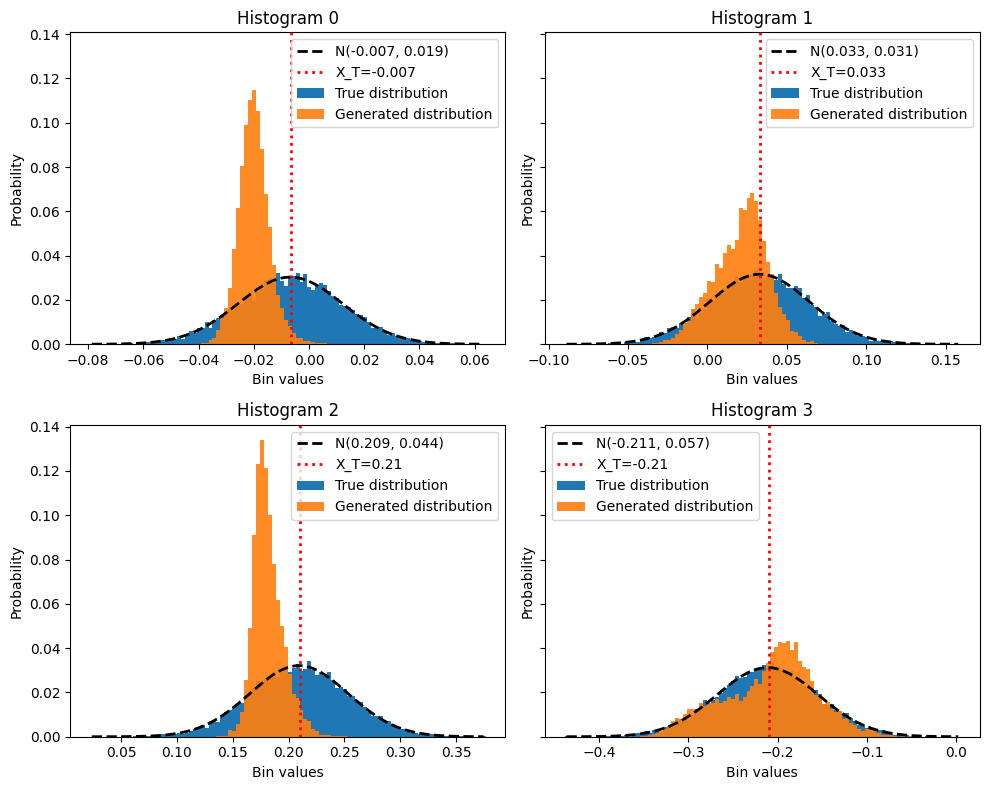
\includegraphics[scale=0.33]{images/samples_forgan_simple.png}
    \caption{Samples obtained from the standard ForGAN using fixed $X_0$ and $\mu$ while varying $\sigma = [0.3, 0.5, 0.7, 0.9]$.}
    \label{forgan_simple_sample_sigma}
\end{figure}
\end{frame}

\begin{frame}{ForGAN vs ForWGAN: Results}
\begin{figure}[H]
    \centering
    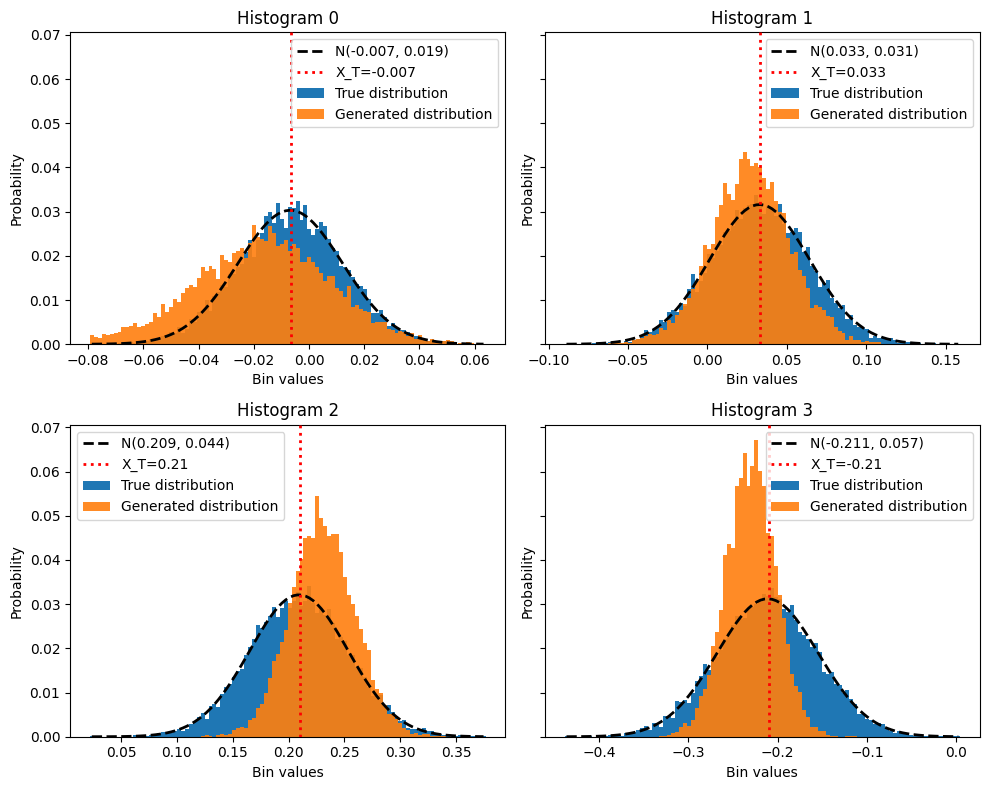
\includegraphics[scale=0.33]{images/samples_forgan.png}
    \caption{Samples obtained from the ForWGAN using fixed $X_0$ and $\mu$ while varying $\sigma = [0.3, 0.5, 0.7, 0.9]$.}
    \label{forwgan_sample_sigma}
\end{figure}

\end{frame}


\begin{frame}{Limitations of GANs}
\textbf{Practical limitations of adversarial training}

\vspace{0.5cm}

\begin{itemize}
    \item \textbf{Non-convergent optimization:}
    the GAN objective is a non-convex two-player game; stochastic
    gradient descent is not guaranteed to converge to the Nash equilibrium.

    \item \textbf{Mode collapse:}
    the generator may concentrate on a small subset of the target
    distribution, failing to reproduce the full probabilistic uncertainty.

    \item \textbf{Underdispersion in forecasting:}
    for a fixed historical condition, different noise draws can produce
    very similar outputs, resulting in a predictive distribution with
    artificially low variance.

    \item \textbf{Vanishing gradients:}
    when the discriminator becomes too effective, the generator may
    receive weak or uninformative gradients precisely when it needs
    corrective feedback.

    \item \textbf{Diversity is not explicitly rewarded:}
    the original adversarial objective provides no direct mechanism
    encouraging the generator to preserve the dispersion of the target
    distribution.
\end{itemize}


\end{frame}


